\documentclass[tikz,border=10pt]{standalone}
\usepackage[T1]{fontenc}
\usepackage{helvet}
\renewcommand{\familydefault}{\sfdefault}
\usetikzlibrary{arrows.meta}

\definecolor{queryfill}{HTML}{DFF7F3}
\definecolor{queryborder}{HTML}{1BA99C}
\definecolor{corpusfill}{HTML}{FFF4D6}
\definecolor{corpusborder}{HTML}{D9A441}
\definecolor{bm25fill}{HTML}{FFE9C8}
\definecolor{bm25border}{HTML}{D88922}
\definecolor{nodefill}{HTML}{E8F2FF}
\definecolor{nodeborder}{HTML}{4E8CD8}
\definecolor{outfill}{HTML}{E7F6E7}
\definecolor{outborder}{HTML}{4FA64F}
\definecolor{softgray}{HTML}{F4F7FB}
\definecolor{darkline}{HTML}{333333}

\tikzset{
  card/.style={rectangle, rounded corners=5pt, align=center, draw=darkline,
               line width=0.8pt, minimum height=1.0cm, font=\small},
  query/.style={card, fill=queryfill, draw=queryborder, minimum width=2.2cm},
  corpus/.style={card, fill=corpusfill, draw=corpusborder, minimum width=2.4cm},
  bm25box/.style={card, fill=bm25fill, draw=bm25border, minimum width=2.9cm},
  artifact/.style={card, fill=white, minimum width=3.0cm},
  output/.style={card, fill=outfill, draw=outborder, minimum width=2.9cm},
  softbox/.style={rectangle, rounded corners=8pt, draw=darkline, fill=softgray, line width=0.7pt},
  leafcirc/.style={circle, fill=nodefill, draw=nodeborder, line width=0.7pt, minimum size=0.32cm},
  rankcirc/.style={circle, fill=outfill, draw=outborder, line width=0.7pt, minimum size=0.32cm},
  phase/.style={font=\small\bfseries, align=center},
  lbl/.style={font=\scriptsize, text=darkline, align=center},
  flow/.style={-{Latex[length=2.4mm]}, line width=0.9pt, draw=darkline},
  divider/.style={dashed, draw=darkline, opacity=0.25, line width=0.7pt}
}

\def\rtop{4.6}
\def\rbot{2.5}
% Query arc y = rtop + card_half (0.5) + 1.20 = 6.30
% Stage headings sit at 6.80, above the arc
\def\arcY{6.30}

\begin{document}
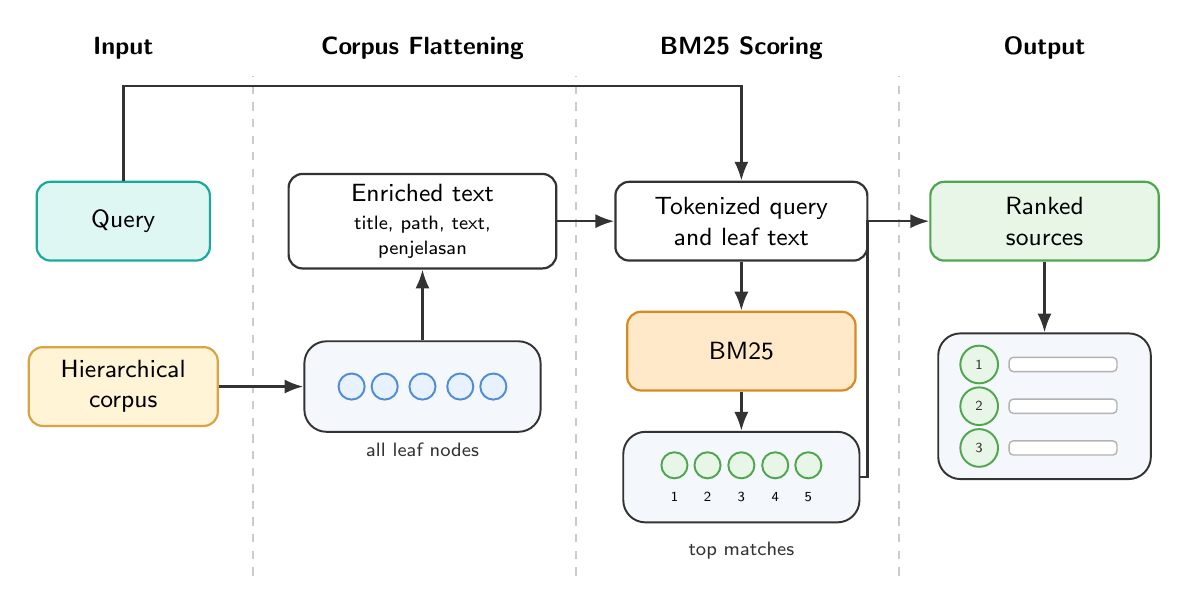
\begin{tikzpicture}

%% Stage headings — above the query arc
\node[phase] at (1.65,  6.80) {Input};
\node[phase] at (5.45,  6.80) {Corpus Flattening};
\node[phase] at (9.50,  6.80) {BM25 Scoring};
\node[phase] at (13.35, 6.80) {Output};

%% Dividers — extend to just below headings
\draw[divider] (3.30,  0.10) -- (3.30,  6.45);
\draw[divider] (7.40,  0.10) -- (7.40,  6.45);
\draw[divider] (11.50, 0.10) -- (11.50, 6.45);

%%  Input
\node[query]  (query)  at (1.65, \rtop) {Query};
\node[corpus] (corpus) at (1.65, \rbot) {Hierarchical\\corpus};

%%  Corpus Flattening
%   Bottom: leaf nodes collected from every document
\node[softbox, minimum width=3.0cm, minimum height=1.15cm] (allnodes) at (5.45, \rbot) {};
\foreach \x in {4.55, 4.97, 5.45, 5.93, 6.35} { \node[leafcirc] at (\x, \rbot) {}; }
\node[lbl] at (5.45, 1.70) {all leaf nodes};

%   Top: per-leaf enriched representation
\node[artifact, minimum width=3.4cm, minimum height=1.2cm] (enriched) at (5.45, \rtop)
  {Enriched text\\[-1pt]{\scriptsize title, path, text,}\\[-2pt]{\scriptsize penjelasan}};

%%  BM25 Scoring
\node[artifact, minimum width=3.2cm] (tokens) at (9.50, \rtop)
  {Tokenized query\\and leaf text};
\node[bm25box] (bm25)   at (9.50, 2.95) {BM25};
\node[softbox, minimum width=3.0cm, minimum height=1.15cm] (ranked) at (9.50, 1.35) {};
\foreach \x/\n in {8.65/1, 9.07/2, 9.50/3, 9.93/4, 10.35/5} {
  \node[rankcirc] at (\x, 1.50) {};
  \node[font=\tiny] at (\x, 1.10) {\n};
}
\node[lbl] at (9.50, 0.42) {top matches};

%%  Output
\node[output] (sources) at (13.35, \rtop) {Ranked\\sources};
\node[softbox, minimum width=2.7cm, minimum height=1.85cm] (rankbox) at (13.35, 2.25) {};
\foreach \y/\n in {2.78/1, 2.25/2, 1.72/3} {
  \node[rankcirc, minimum size=0.36cm, font=\tiny, text=darkline] at (12.52, \y) {\n};
  \filldraw[rounded corners=1.5pt, fill=white, draw=black!30, line width=0.5pt]
    (12.90, \y-0.09) rectangle (14.27, \y+0.09);
}

%%  Flow
% Corpus → leaf nodes
\draw[flow] (corpus.east) -- (allnodes.west);
% Leaf nodes → enriched text (upward)
\draw[flow] (allnodes.north) -- (enriched.south);
% Enriched text → tokenization
\draw[flow] (enriched.east) -- (tokens.west);
% Query arcs north above all content, then down into tokenization
% Arc height = \arcY = 6.30, well above enriched.north (~5.2) and below headings (6.80)
\draw[flow] (query.north) -- ++(0, 1.20) -| (tokens.north);
% Scoring chain
\draw[flow] (tokens.south) -- (bm25.north);
\draw[flow] (bm25.south)   -- (ranked.north);
% Top matches rise to ranked sources — riser at x=11.10 gives 0.80 cm approach
\draw[flow] (ranked.east) -- (11.10, 1.35) -- (11.10, \rtop) -- (sources.west);
% Ranked sources → numbered list
\draw[flow] (sources.south) -- (rankbox.north);

\end{tikzpicture}
\end{document}
